\documentclass[12pt]{article}

\usepackage[a4paper,margin=1in]{geometry}
\usepackage{amsmath}
\usepackage{amssymb}
\usepackage{enumitem}
\usepackage{physics}
\usepackage{tikz}
\usetikzlibrary{
    arrows.meta,
    calc,
    angles,
    quotes,
    decorations.pathmorphing
}


\setlist[enumerate]{itemsep=1.6em}

\begin{document}

\begin{center}
\Large \textbf{PAPER 4 – ULTRA HARD VERSION}\\
\large Electrostatics | Current Electricity | Electromagnetic Induction\\
\large (Single Correct Type – 4 Options Each)
\end{center}

\vspace{0.5cm}

\begin{enumerate}

% ================= ELECTROSTATICS =================

\item Two point charges $+q$ and $-q$ are fixed at coordinates $(0,a)$ and $(0,-a)$ respectively, forming a dipole of moment $\vec p$. A point $P$ lies on the positive $x$-axis at a distance $x$ from the origin such that $x \gg a$.

Using binomial expansion up to the lowest non-vanishing order and resolving vector components carefully, determine the leading-order magnitude of the electric field at $P$. Also identify its direction relative to dipole axis.

\begin{enumerate}[label=\Alph*)]
\item $\dfrac{1}{4\pi\epsilon_0}\dfrac{2qa}{x^3}$ directed along negative $y$-axis
\item $\dfrac{1}{4\pi\epsilon_0}\dfrac{qa}{x^3}$ directed along positive $x$-axis
\item $\dfrac{1}{4\pi\epsilon_0}\dfrac{2qa}{x^2}$ directed along negative $x$-axis
\item $\dfrac{1}{4\pi\epsilon_0}\dfrac{q}{x^2}$ directed along positive $y$-axis
\end{enumerate}

\item A thin circular ring of radius $R$ carries uniform charge $Q$. A point $P$ lies on its axis at distance $x$.

Derive the exact expression for the electric field using symmetry and integration. Then determine the condition for which the magnitude of electric field becomes maximum with respect to $x$.

% ================= Q2 DIAGRAM =================
\begin{center}
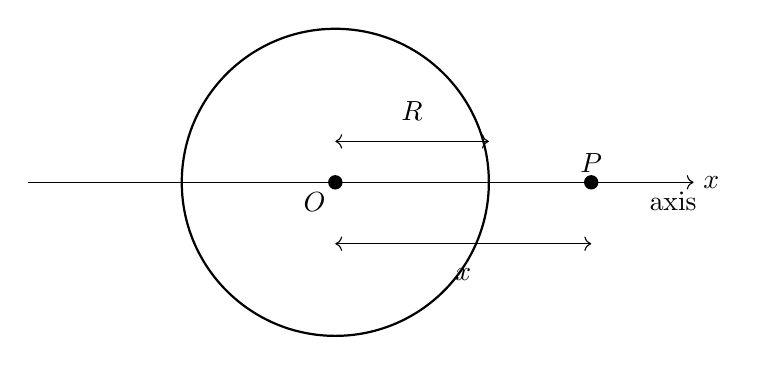
\begin{tikzpicture}[scale=1.3]

% Ring
\draw[thick] (0,0) circle (1.5);

% Axis
\draw[->] (-3,0) -- (3.5,0) node[right] {$x$};
\node[below] at (3.3,0) {axis};

% Center
\fill (0,0) circle (2pt);
\node[below left] at (0,0) {$O$};

% Point P
\fill (2.5,0) circle (2pt);
\node[above] at (2.5,0) {$P$};

% Distance x
\draw[<->] (0,-0.6) -- (2.5,-0.6);
\node at (1.25,-0.9) {$x$};

% Radius R
\draw[<->] (0,0.4) -- (1.5,0.4);
\node at (0.75,0.7) {$R$};

\end{tikzpicture}
\end{center}

\begin{enumerate}[label=\Alph*)]
\item $\dfrac{1}{4\pi\epsilon_0}\dfrac{Qx}{(R^2+x^2)^{3/2}}$, maximum at $x = \dfrac{R}{\sqrt{2}}$
\item $\dfrac{1}{4\pi\epsilon_0}\dfrac{Q}{R^2+x^2}$, maximum at $x = R$
\item $\dfrac{1}{4\pi\epsilon_0}\dfrac{Qx}{(R^2+x^2)^{3/2}}$, maximum at $x = R$
\item $\dfrac{1}{4\pi\epsilon_0}\dfrac{Q}{x^2}$, maximum at $x \to 0$
\end{enumerate}

\item Two identical conducting spheres carry charges $Q$ and $-Q$. They are brought into contact via a thin conducting wire while remaining fixed in space. The system is isolated.

Taking into account electrostatic induction, charge flow through the wire, and energy minimization arguments, determine the final charge distribution on the spheres after equilibrium is established.

\begin{enumerate}[label=\Alph*)]
\item $Q, -Q$
\item $0, 0$
\item $Q/2, -Q/2$
\item Depends on separation
\end{enumerate}

\item A parallel plate capacitor (plate area $A$, separation $d$) is connected to a battery of emf $V$. A dielectric slab of dielectric constant $K$ partially fills the region and is slowly withdrawn while battery remains connected.

Considering fringing negligible, determine which quantity decreases during the process.

% ================= Q4 DIAGRAM =================
\begin{center}
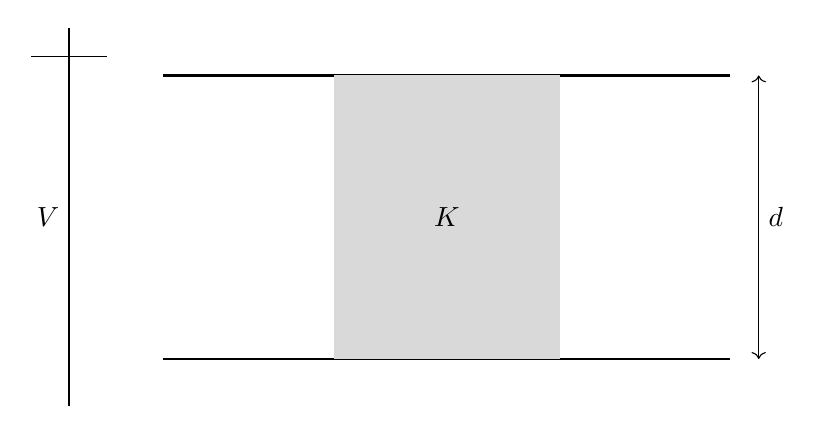
\begin{tikzpicture}[scale=1.2]

% Plates
\draw[thick] (-3,1.5) -- (3,1.5);
\draw[thick] (-3,-1.5) -- (3,-1.5);

% Battery
% Battery (proper symbol)
\draw (-4,2) -- (-4,1);        % long plate
\draw (-4.4,1.7) -- (-3.6,1.7); % short plate
\draw (-4,1) -- (-4,-1);
\draw (-4,-1) -- (-4,-2);
\node[left] at (-4,0) {$V$};

% Dielectric slab
\fill[gray!30] (-1.2,-1.5) rectangle (1.2,1.5);
\node at (0,0) {$K$};

% Separation d
\draw[<->] (3.3,-1.5) -- (3.3,1.5);
\node[right] at (3.3,0) {$d$};

\end{tikzpicture}
\end{center}

\begin{enumerate}[label=\Alph*)]
\item Capacitance only
\item Charge on plates only
\item Electric field between plates
\item Potential difference across plates
\end{enumerate}

\item A dipole of moment $\vec p$ making an arbitrary angle with the $x$-axis is placed in a spatially varying electric field $\vec E = kx \hat i$.

Derive expressions for both torque and net force on the dipole. Under what condition does the dipole experience translational acceleration in addition to rotation?

\begin{enumerate}[label=\Alph*)]
\item Only torque exists
\item Only force exists
\item Both force and torque exist
\item Neither force nor torque exists
\end{enumerate}

% ================= CURRENT ELECTRICITY =================

\item A metallic wire of resistance $R$, length $L$, and area $A$ is stretched to twice its length while maintaining constant volume.

Assuming resistivity remains constant, derive the new resistance.

\begin{enumerate}[label=\Alph*)]
\item $2R$
\item $4R$
\item $8R$
\item $R/2$
\end{enumerate}

\item A cell of emf $E$ and internal resistance $r$ is connected to a variable external resistance $R$.

Using differentiation, determine the value of $R$ for which power delivered to external resistor is maximum.

\begin{enumerate}[label=\Alph*)]
\item $R = r$
\item $R = 2r$
\item $R = r/2$
\item $R \to \infty$
\end{enumerate}

\item A resistor follows non-linear characteristic $V = aI^2$ for $V \ge 0$ and does not conduct for negative applied voltage. The applied voltage varies sinusoidally as $V = V_0 \sin \omega t$.
Determine the nature of current waveform and its frequency components.

% ================= Q8 DIAGRAM =================
\begin{center}
\begin{tikzpicture}[scale=1.1]

% Axes
\draw[->] (0,0) -- (6.5,0) node[right] {$t$};
\draw[->] (0,-2.2) -- (0,2.2) node[above] {$V$};

% Sinusoidal voltage
\draw[thick,domain=0:6,samples=200]
plot (\x,{1.5*sin(60*\x)});

\node at (5.5,1.5) {$V_0 \sin \omega t$};

\end{tikzpicture}
\end{center}

\begin{enumerate}[label=\Alph*)]
\item Purely sinusoidal of frequency $\omega$
\item Contains harmonic components (multiple frequencies)
\item Constant magnitude
\item Zero for half cycle
\end{enumerate}

\item An infinite network of resistors is formed such that each section consists of one resistor $R$ in series followed by one resistor $R$ in parallel with remaining network.

Using self-consistency method, determine equivalent resistance between input terminals.

\begin{enumerate}[label=\Alph*)]
\item $R$
\item $\dfrac{1+\sqrt{5}}{2}R$
\item $\dfrac{R}{2}$
\item $\sqrt{2}R$
\end{enumerate}

\item Using classical electron theory, drift velocity is given in terms of relaxation time.

Analyze how drift velocity changes with temperature assuming relaxation time decreases with increasing lattice vibrations.

\begin{enumerate}[label=\Alph*)]
\item Increases with temperature
\item Decreases with temperature
\item Remains constant
\item Depends on length of conductor
\end{enumerate}

% ================= ELECTROMAGNETIC INDUCTION =================

\item A conducting rod of length $l$ rotates with constant angular velocity $\omega$ about one end in a uniform magnetic field perpendicular to plane of rotation.

Using elemental emf approach and integration, determine induced emf between its ends.

% ================= Q11 DIAGRAM =================
\begin{center}
\begin{tikzpicture}[scale=1.2]

% Pivot
\fill (0,0) circle (2pt);

% Rod
\draw[thick] (0,0) -- (3,1.5);
\node[right] at (3,1.5) {$l$};

% Angular velocity arrow
\draw[->] (0.6,0.2) arc (20:70:0.8);
\node at (1.2,0.8) {$\omega$};

% Magnetic field dots
\foreach \x in {-2,-1,0,1,2}
  \foreach \y in {-2,-1,0,1,2}
    \draw (\x,\y) circle (0.05);

\node[right] at (3.2,-1.5) {$B$ (out of page)};

\end{tikzpicture}
\end{center}

\begin{enumerate}[label=\Alph*)]
\item $\dfrac{1}{2}B\omega l^2$
\item $B\omega l^2$
\item $Bl\omega$
\item Zero
\end{enumerate}

\item A circular conducting loop of variable radius lies in uniform magnetic field perpendicular to plane. The radius increases at constant rate while magnetic field remains constant.

Determine direction of induced current.

% ================= Q12 DIAGRAM =================
\begin{center}
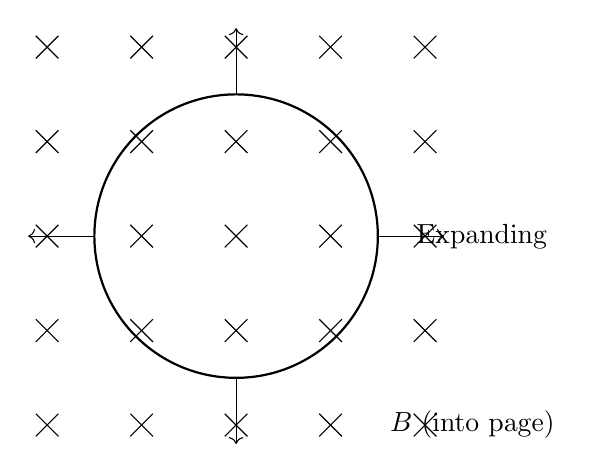
\begin{tikzpicture}[scale=1.2]

% Loop
\draw[thick] (0,0) circle (1.5);

% Expansion arrows
\draw[->] (1.5,0) -- (2.2,0);
\draw[->] (-1.5,0) -- (-2.2,0);
\draw[->] (0,1.5) -- (0,2.2);
\draw[->] (0,-1.5) -- (0,-2.2);

\node at (2.6,0) {Expanding};

% Magnetic field crosses
\foreach \x in {-2,-1,0,1,2}
  \foreach \y in {-2,-1,0,1,2}
  {
    \draw (\x-0.12,\y-0.12) -- (\x+0.12,\y+0.12);
    \draw (\x-0.12,\y+0.12) -- (\x+0.12,\y-0.12);
  }

\node at (2.5,-2) {$B$ (into page)};

\end{tikzpicture}
\end{center}

\begin{enumerate}[label=\Alph*)]
\item Clockwise
\item Anticlockwise
\item Zero
\item Depends on rate of expansion
\end{enumerate}

\item A coil of $N$ turns experiences magnetic flux changing from $\Phi_1$ to $\Phi_2$ in time $\Delta t$.

Determine magnitude of induced emf.

\begin{enumerate}[label=\Alph*)]
\item $N\dfrac{\Phi_2-\Phi_1}{\Delta t}$
\item $\dfrac{\Phi_2-\Phi_1}{\Delta t}$
\item $\dfrac{1}{N}\dfrac{\Phi_2-\Phi_1}{\Delta t}$
\item Zero
\end{enumerate}

\item Using energy conservation principle, identify the fundamental reason why induced current always opposes change in magnetic flux.

\begin{enumerate}[label=\Alph*)]
\item Charge conservation
\item Energy conservation
\item Momentum conservation
\item Ohm’s law
\end{enumerate}

\item A long solenoid of length $l$, cross-sectional area $A$, and $n$ turns per unit length carries current $I$.

Determine which factors self-inductance depends upon.

\begin{enumerate}[label=\Alph*)]
\item Current only
\item Geometry and permeability of medium
\item Resistance only
\item Applied voltage
\end{enumerate}

\end{enumerate}

\end{document}